\documentclass[a4paper,12pt]{article}
\usepackage[dutch]{babel}
\usepackage{graphicx}
\usepackage{float}

\usepackage{multicol}
\setlength{\columnsep}{1cm}

\begin{document}
\title{Een persoonlijk verslag naar de afhandeling van beoordelingssystemiek in geavanceerde algoritmen}
\author{Galvin Bartes}
\maketitle
\tableofcontents
\begin{table}[h] % drijvende tabel
\caption{States voor Uppaal model.} % bijschrift, wordt automatisch genummerd
\label{reqs} % label om naar figuur te verwijzen
\begin{center} % centreer de tabel
\begin{tabular}{llc} % 3 kolommen, 2 links uitgelijnd en 1 gecentreerd
\hline % horizontale lijn
\textbf{Nr.} & \textbf{Item} & \textbf{MoSCoW}\\ % kolommen gescheiden met &
\hline
1 & Schip A komt aan van links en communiceert met Sluis & M\\
1b) & Schip B komt aan van rechts en cmmuniceert met Sluis & S\\
aanname & Sluis is leeg & M\\
aanname & sluisdeuren 1,2,3,4 zijn dicht & S\\
2) & kade stuurt signal naar schip A, mag komen & S\\
3) & Schip A komt aan & S\\
4) & Kade stuurt signal naar schip B, schip B moet wachten & S\\
5) & Schip B gaat afremmen & S\\
6) & Schip B is afgeremd voor deur 3 & S\\
7) & Schip A krijgt signal sluis deur 1 en 2 gaan open & S\\
8) & sluis deur 1 en 2 zijn geopend & S\\
9) & Schip A in sluis, sluis A moet afremmen & S\\
10) & Schip A gestopt bij ingang van deur drie & S\\
11) & Deuren 1 en 2 sluiten & S\\
12) & Deuren 1 en 2 gesloten & S\\
13) & Nog ruimte voor nog een ship, kade signaleert schip B voor deur 4 & S\\
14) & Deur 4 gaat open & S\\
15) & deur 4 is geopend & S\\
16) & Schip B start op geeft gas, stuurt bij en kiest deur & S\\
17) & Schip B afremmen & S\\
18) & Schip B gestopt & S\\

19) & Sluisdeur sluiten & S\\
20) & Sluisdeur gesloten & S\\

\hline
\end{tabular}
\end{center}
\end{table}



\begin{table}[h] % drijvende tabel
\caption{States voor Uppaal model.} % bijschrift, wordt automatisch genummerd
\label{reqs} % label om naar figuur te verwijzen
\begin{center} % centreer de tabel
\begin{tabular}{llc} % 3 kolommen, 2 links uitgelijnd en 1 gecentreerd
\hline % horizontale lijn
\textbf{Nr.} & \textbf{Item} & \textbf{MoSCoW}\\ % kolommen gescheiden met &
\hline
21) & Sensor aan & S\\
22) & sensor geeft hoogte water door aan kade & S\\
23) & controller stelt gewenste hoogte voor water bij & S\\
24) & pomp activeren & S\\
25) & pomp geactiveerd & S\\
26) & Sensor hoogte water meten & S\\
27) & Water hoogte gemeten & S\\
aanname: & eerste keer meten is succesvol & S\\
28) &  Sluisdeuren mogen open & S\\
29) &  Sluisdeur 2 en 3 zijn geopend & S\\
20) &  Schip A en B opstarten & S\\
21) & Schip A en B opgestart en rijden weg, verdwijnen uit model & S\\
22) & Volgende Schip uit wachtrij wordt in model gebracht & S\\
23  & Kost weinig & C\\

\hline
\end{tabular}
\end{center}
\end{table}

\section{Verklarende begrippen}

\begin{multicols}{2}
[
\section{First Section}
De rol van functionele eisen

]

\begin{itemize}
  \item Functionele eis definities:
  \item Niet-Functionele eis definities:
\end{itemize}


\end{multicols}
 



\section{samenvatting}

Logica

Theoretische informatica



\section{Inleiding\dots}
Aanleiding voor het onderzoek
\begin{figure}
    \centering
    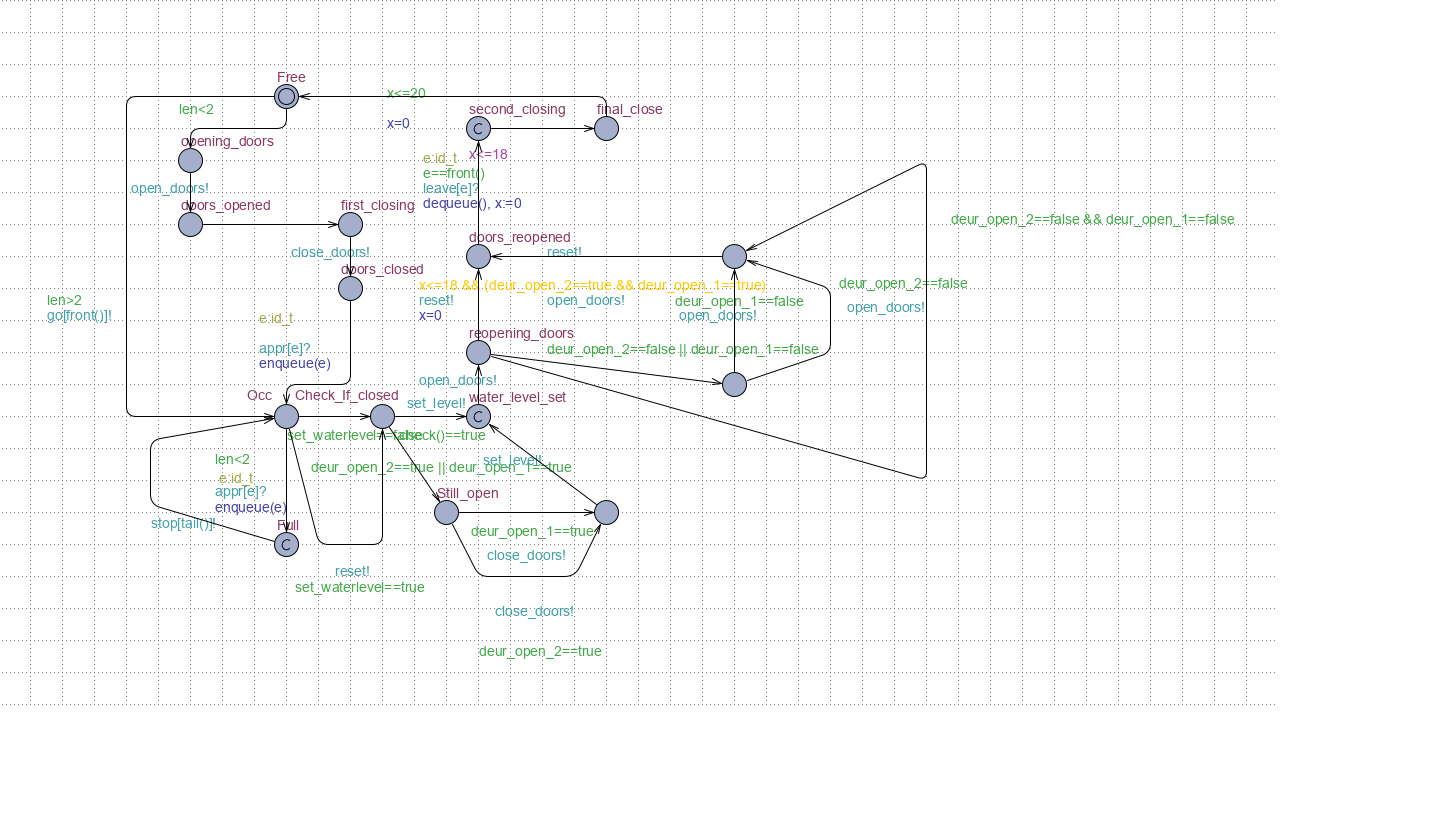
\includegraphics[width=2.5\textwidth]{Controller.png}
    \caption{Controller}
    \label{fig:figuur_1}
\end{figure}

\begin{figure}
    \centering
    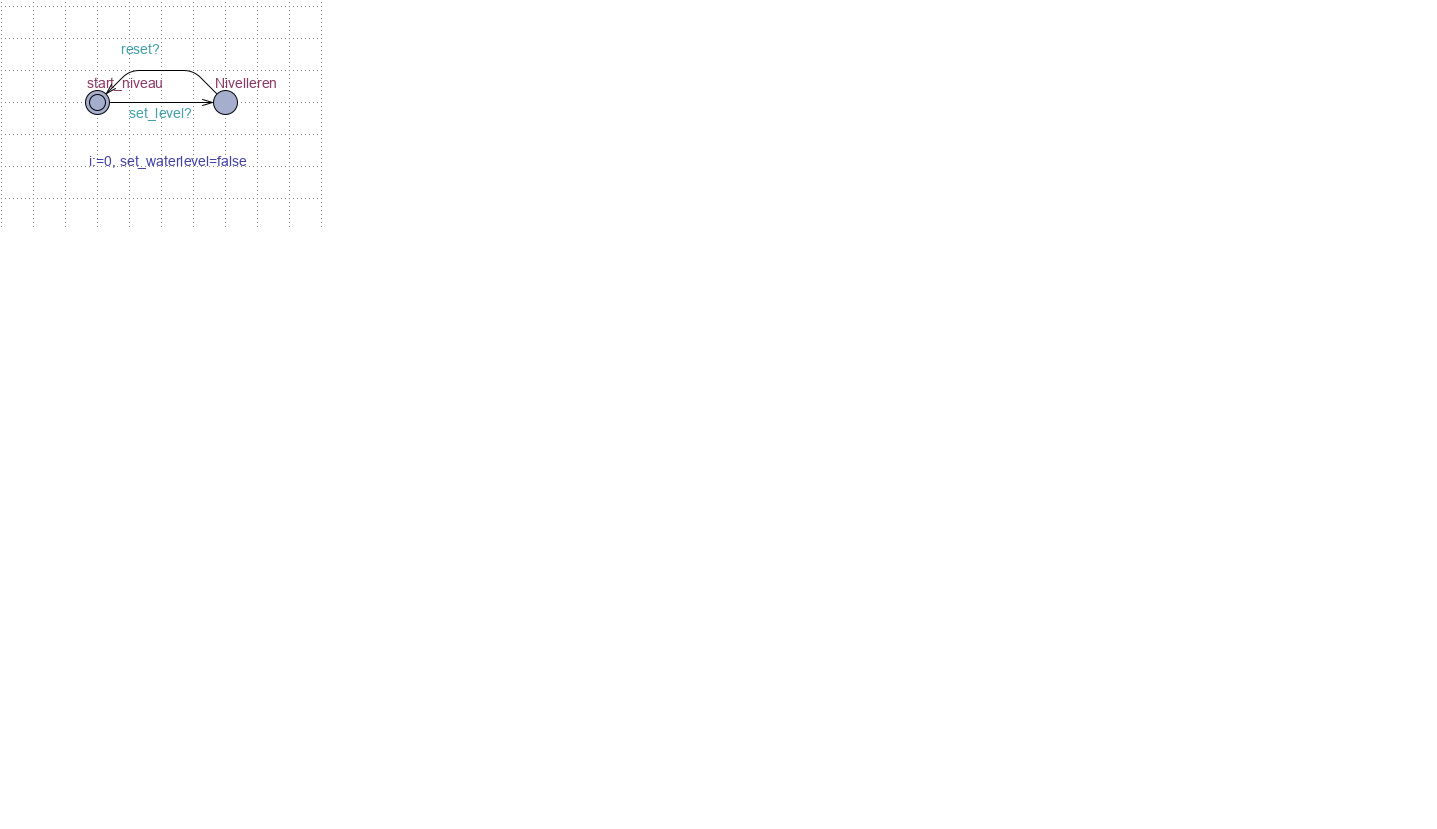
\includegraphics[width=2.5\textwidth]{nivelleer_nieuw.png}
    \caption{nivelleer}
    \label{fig:figuur_2}
\end{figure}

\ref{figuur_1}
Random citation \cite{Nobody06} embeddeed in text.
\section{Probleemstelling\dots}
\section{Research\dots}

Mode confusion: bij de mens is verwarring over de daadwerkeljike systeemtoestand

Automatiseringsparadox: bij toenemende automatisering wordt het menselijk ingrijpen steeds crucialer door de impac en complexiteit van het systeem

\section{Conclusion\dots}\newpage
\section{Discussion\dots}
\bibliography{mybibliography}{}
\bibliographystyle{plain}

\begin{thebibliography}{9}
\bibitem{texbook}
Donald E. Knuth (1986) \emph{The \TeX{} Book}, Addison-Wesley Professional.

\bibitem{lamport94}
Leslie Lamport (1994) \emph{\LaTeX: a document preparation system}, Addison
Wesley, Massachusetts, 2nd ed.




\bibitem{lamport94}
Leslie Lamport (1994) \emph{\LaTeX: a document preparation system}, Addison
Wesley, Massachusetts, 2nd ed.



\bibitem{lamport94}
http://www.sts.tu-harburg.de/pw-and-m-theses/2012/rinas12.pdf

\bibitem{lamport94}
http://www.sts.tu-harburg.de/pw-and-m-theses/2012/rinas12.pdf
\bibitem{lamport94}
http://people.cs.aau.dk/~adavid/publications/21-tutorial.pdf
\bibitem{lamport94}
http://www.artist-embedded.org/docs/Events/2011/Aix-les-Bains/Presentations/1-Sunday/Kim_Larsen.pdf
\bibitem{lamport94}
https://conservancy.umn.edu/bitstream/handle/11299/190597/Vuppula_umn_0130M_18273.pdf?sequence=1
\bibitem{lamport94}
http://www.avacs.org/fileadmin/Publikationen/Open/dierks05.pdf
\bibitem{lamport94}
https://ori-nuxeo.univ-lille1.fr/nuxeo/site/esupversions/9799b42e-643f-4443-b330-5321cc08b9f4
\bibitem{lamport94}
http://www.hessel.nu/CoVer/publications/frst_Master.pdf
\bibitem{lamport94}
http://ntur.lib.ntu.edu.tw/bitstream/246246/44838/1/01316040.pdf
\bibitem{lamport94}
https://www.mi.fu-berlin.de/inf/groups/ag-tech/intern/19548-V-Model-Checking/Pettersson__Paul.pdf
\bibitem{lamport94}
https://ori-nuxeo.univ-lille1.fr/nuxeo/site/esupversions/9799b42e-643f-4443-b330-5321cc08b9f4
\bibitem{lamport94}
https://www.researchgate.net/publication/221352048_Testing_real-time_systems_using_UPPAAL

\bibitem{lamport94}
https://pdfs.semanticscholar.org/95e4/3f685c92dcdcc735cc6aed28aee4f9a05c40.pdf
\bibitem{lamport94}
https://www.sws.cs.ru.nl/publications/papers/fvaan/DynamicUppaal/FSEN13.pdf
\bibitem{lamport94}
https://backend.orbit.dtu.dk/ws/portalfiles/portal/197983400/main_timetable_mc2019.pdf
\bibitem{lamport94}
https://www.researchgate.net/profile/Stephan_Merz/publication/221654839_Model_Checking_Timed_UML_State_Machines_and_Collaborations/links/0046351a617959cf27000000/Model-Checking-Timed-UML-State-Machines-and-Collaborations.pdf
\bibitem{lamport94}
https://aleksdimovski.github.io/files/kimfest17.pdf
\bibitem{lamport94}
https://www.researchgate.net/publication/4357738_Verification_and_Implementation_of_Dependable_Controllers
\bibitem{lamport94}
http://erasmusmundus.ie/courses/desem/sites/default/files/Modelling%20and%20Transformation%20of%20Non-Functional%20Annotations.pdf
\bibitem{lamport94}
https://inf.mit.bme.hu/sites/default/files/materials/category/kateg%C3%B3ria/oktat%C3%A1s/v%C3%A1laszthat%C3%B3-t%C3%A1rgyak/kritikus-be%C3%A1gyazott-rendszerek/15/05_Formal_modelling_verification.pdf
\bibitem{lamport94}
http://people.cs.aau.dk/~ask/MTV/material/rt-uppaal.pdf
\bibitem{lamport94}
http://erasmusmundus.ie/courses/desem/sites/default/files/Modelling%20and%20Transformation%20of%20Non-Functional%20Annotations.pdf
\bibitem{lamport94}
https://www.sciencedirect.com/science/article/abs/pii/S0166361515300178
\bibitem{lamport94}






\end{thebibliography}

\end{document}


